\begin{frame}
  \begin{center}
    \Huge Algorithm
  \end{center}
\end{frame}

\begin{frame}
  \frametitle{Algorithm}
  \framesubtitle{Notations}
  Let
  \begin{itemize}
    \item \blue{$\Lambda_i$} be the list of labels on node \blue{$i \in V$};
    \item \blue{$N$} be the list of nodes to be processed;
    \item \blue{\[
        f(S_i) =  
        \begin{cases}
          \text{\textcolor{black}{true}},  & \text{\textcolor{black}{if} }      \forall r \in R (l_i^r \leqslant e_i^r) \wedge \forall j \in V (v_i^j \leqslant 1)\\
          \text{\textcolor{black}{false}}, & \text{\textcolor{black}{otherwise}}
        \end{cases}
    \]} be a function that says whether a label is feasible;
\item \blue{$ E(S_i, j) = (\text{max} \{l^r_i + d_{ij}^r, b^r_j\} : r \in R) \cup (s_i + 1, v_i^1, ..., v_i^j + 1, $} \blue{$..., v_i^{|V|}) $} be the function that returns the label resulting from the extension of a path \blue{$P_i$} by a node \blue{$j$};
    \item \blue{$F_{ij}$} be the set of labels extended from \blue{$i$} to \blue{$j \in V$}; and
    \item \blue{$N_D(\Lambda) = \{S_i \in \Lambda : \nexists S^{'}_i \in \Lambda (S^{'}_i \neq S_i \wedge S^{'}_i \leqslant S_i) \}$} be the function that returns all nondominated labels from \blue{$\Lambda$}.
  \end{itemize}
\end{frame}

\begin{frame}
  \frametitle{Algorithm}
  \framesubtitle{Code}
  \begin{algorithm}[H]
    \scriptsize
    \begin{algorithmic}[1]
      \REQUIRE \blue{$D(V, A), c_a \quad \forall a \in A, d_a^r \quad \forall a \in A, r \in R$}
      %initialization
      \STATE \blue{$\Lambda_s \gets \{ (\{0\}^{|R|} \cup (1, 1) \cup \{0\}^{|V| - 1}, 0) \}$};
      \STATE \blue{$\Lambda_i \gets \emptyset \quad \forall i \in V \backslash \{s\}$};
      \STATE \blue{$N \gets \{s\}$};
      %exploration
      \label{step:main_while}\WHILE {\blue{$N \neq \emptyset$}}
        \STATE Let \blue{$i \in N$} be a \blue{$N$} arbitrary node;
        \label{step:explore_arcs}\FORALL {\blue{$(i, j) \in \delta^{+}(i)$}}
          \STATE \blue{$F_{ij} \gets \emptyset$};
          \FORALL {\blue{$S_i \in \Lambda_i$}}
            \IF {\blue{$f(E(S_i, j))$}}
              \STATE \blue{$F_{ij} \gets F_{ij} \cup \{E(S_i, j)\}$};
            \ENDIF
          \ENDFOR
          \STATE \blue{$\Lambda_j \gets N_D(F_{ij} \cup \Lambda_j)$};
          \IF {\blue{$\Lambda_j$} has changed}
            \STATE \blue{$N \gets N \cup \{j\}$};
          \ENDIF
        \ENDFOR
        \STATE \blue{$N \gets N \backslash \{i\}$};
      \ENDWHILE
      \RETURN \blue{min$_{(L_t, C_t) \in \Lambda_t} \{ C_t \}$} if \blue{$\Lambda_t \neq \emptyset$} else \blue{$\infty$};
    \end{algorithmic}
    \caption{Labeling algorithm}
    \label{alg:seq}
  \end{algorithm}
\end{frame}

\begin{frame}
  \frametitle{Algorithm}
  \framesubtitle{Example}
  \begin{multicols}{2}
    State before line \ref{step:main_while}:
    \begin{itemize}   
      \item \blue{$\Lambda_s = \{ ((0, 0, 1, 1, 0, 0, 0), 0) \}$};
      \item \blue{$\Lambda_2 = \Lambda_3 = \Lambda_t = \emptyset$};
      \item \blue{$N = \{\{s\}\}$};
    \end{itemize}   
    \begin{figure}[H]
      \centering
      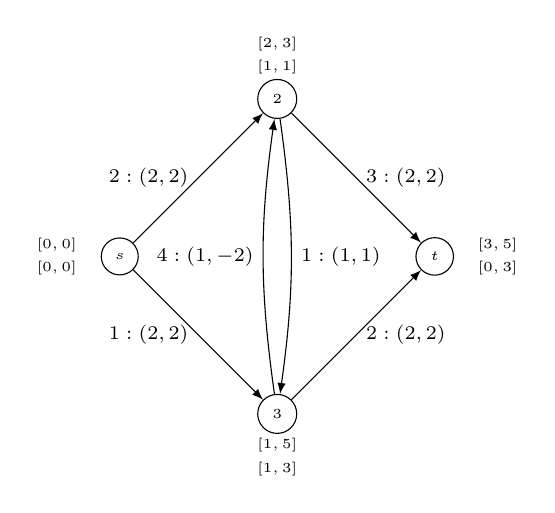
\begin{tikzpicture}[font=\tiny]
        %nodes
        \node at (-0.8, 0.15) {\blue{$[0,0]$}};
        \node at (-0.8, -0.15) {\blue{$[0,0]$}};
        \node[circle, draw] (s) at (0, 0) {\blue{$s$}};
        \node at (2, 2.7) {\blue{$[2, 3]$}};
        \node at (2, 2.4) {\blue{$[1, 1]$}};
        \node[circle, draw] (a) at (2, 2) {\blue{$2$}};
        \node at (2, -2.4) {\blue{$[1, 5]$}};
        \node at (2, -2.7) {\blue{$[1, 3]$}};
        \node[circle, draw] (b) at (2, -2) {\blue{$3$}};
        \node at (4.8, 0.15) {\blue{$[3, 5]$}};
        \node at (4.8, -0.15) {\blue{$[0, 3]$}};
        \node[circle, draw] (t) at (4, 0) {\blue{$t$}};
        %edges
        \path [draw,-latex] (s) to node[left]{\scriptsize\blue{$2: (2, 2)$}} (a);
        \path [draw,-latex] (s) to node[left]{\scriptsize\blue{$1: (2, 2)$}} (b);
        \path [draw,-latex] (a) to node[right]{\scriptsize\blue{$3: (2, 2)$}} (t);
        \path [draw,-latex] (b) to node[right]{\scriptsize\blue{$2: (2, 2)$}} (t);
        \path [draw,-latex] (a) edge [bend left=8] node[right]{\scriptsize\blue{$1: (1, 1)$}} (b);
        \path [draw,-latex] (b) edge [bend left=8] node[left]{\scriptsize\blue{$4: (1, -2)$}} (a);
      \end{tikzpicture}
      \caption{A ERCSPP instance digraph example.}
    \end{figure}
  \end{multicols}
\end{frame}

\begin{frame}
  \frametitle{Algorithm}
  \framesubtitle{Example}
  \begin{multicols}{2}
    State at the end of \blue{$1$}st iteration of the while at line \ref{step:main_while}:
    \begin{itemize}   
      \item \blue{$\Lambda_s = \{ ((0, 0, 1, 1, 0, 0, 0), 0) \}$};
      \item \blue{$\Lambda_2 = \emptyset$};
      \item \blue{$\Lambda_3 = \{((2, 2, 2, 1, 0, 1, 0), 1)\}$};
      \item \blue{$\Lambda_t = \emptyset$};
      \item \blue{$N = \{\{3\}\}$};
    \end{itemize}   
    \begin{figure}[H]
      \centering
      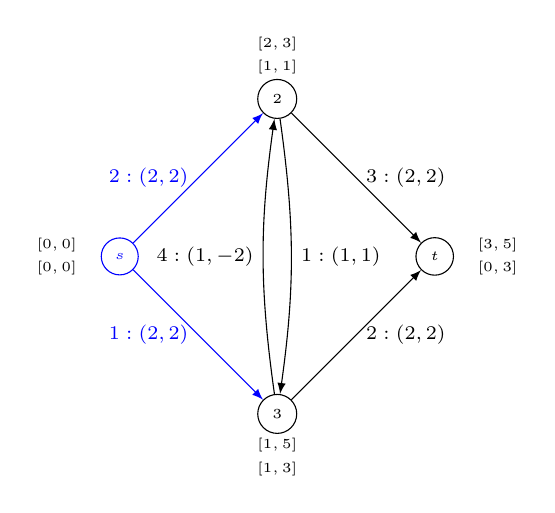
\begin{tikzpicture}[font=\tiny]
        %nodes
        \node at (-0.8, 0.15) {\blue{$[0,0]$}};
        \node at (-0.8, -0.15) {\blue{$[0,0]$}};
        \node[blue, circle, draw] (s) at (0, 0) {\blue{$s$}};
        \node at (2, 2.7) {\blue{$[2, 3]$}};
        \node at (2, 2.4) {\blue{$[1, 1]$}};
        \node[circle, draw] (a) at (2, 2) {\blue{$2$}};
        \node at (2, -2.4) {\blue{$[1, 5]$}};
        \node at (2, -2.7) {\blue{$[1, 3]$}};
        \node[circle, draw] (b) at (2, -2) {\blue{$3$}};
        \node at (4.8, 0.15) {\blue{$[3, 5]$}};
        \node at (4.8, -0.15) {\blue{$[0, 3]$}};
        \node[circle, draw] (t) at (4, 0) {\blue{$t$}};
        %edges
        \path [blue, draw,-latex] (s) to node[left]{\scriptsize\blue{$2: (2, 2)$}} (a);
        \path [blue, draw,-latex] (s) to node[left]{\scriptsize\blue{$1: (2, 2)$}} (b);
        \path [draw,-latex] (a) to node[right]{\scriptsize\blue{$3: (2, 2)$}} (t);
        \path [draw,-latex] (b) to node[right]{\scriptsize\blue{$2: (2, 2)$}} (t);
        \path [draw,-latex] (a) edge [bend left=8] node[right]{\scriptsize\blue{$1: (1, 1)$}} (b);
        \path [draw,-latex] (b) edge [bend left=8] node[left]{\scriptsize\blue{$4: (1, -2)$}} (a);
      \end{tikzpicture}
      \caption{Arcs explored the for loop at line \ref{step:explore_arcs} when \blue{$i = s$}.}
      \label{fig:vrptw_disposable_example}
    \end{figure}
  \end{multicols}
\end{frame}

\begin{frame}
  \frametitle{Algorithm}
  \framesubtitle{Example}
  \begin{multicols}{2}
    State at the end of \blue{$2$}rd iteration of the while at line \ref{step:main_while}:
    \begin{itemize}   
      \item \blue{$\Lambda_s = \{ ((0, 0, 1, 1, 0, 0, 0), 0) \}$};
      \item \blue{$\Lambda_2 = \{((3, 0, 3, 1, 1, 1, 0), 5)\}$};
      \item \blue{$\Lambda_3 = \{((2, 2, 2, 1, 0, 1, 0), 1)\}$};
      \item \blue{$\Lambda_t = \emptyset$};
      \item \blue{$N = \{\{2\}\}$};
    \end{itemize}   
    \begin{figure}[H]
      \centering
      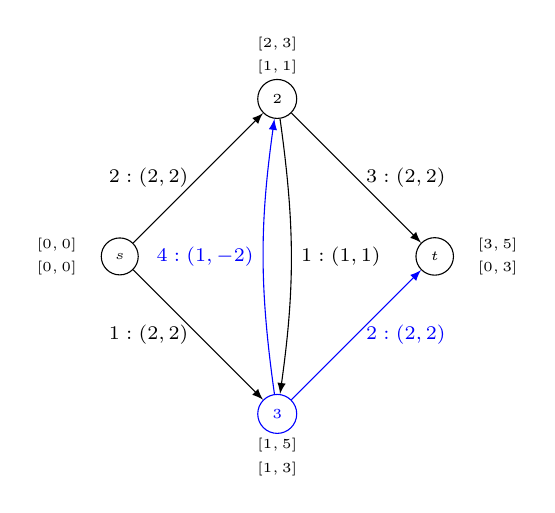
\begin{tikzpicture}[font=\tiny]
        %nodes
        \node at (-0.8, 0.15) {\blue{$[0,0]$}};
        \node at (-0.8, -0.15) {\blue{$[0,0]$}};
        \node[circle, draw] (s) at (0, 0) {\blue{$s$}};
        \node at (2, 2.7) {\blue{$[2, 3]$}};
        \node at (2, 2.4) {\blue{$[1, 1]$}};
        \node[circle, draw] (a) at (2, 2) {\blue{$2$}};
        \node at (2, -2.4) {\blue{$[1, 5]$}};
        \node at (2, -2.7) {\blue{$[1, 3]$}};
        \node[blue, circle, draw] (b) at (2, -2) {\blue{$3$}};
        \node at (4.8, 0.15) {\blue{$[3, 5]$}};
        \node at (4.8, -0.15) {\blue{$[0, 3]$}};
        \node[circle, draw] (t) at (4, 0) {\blue{$t$}};
        %edges
        \path [draw,-latex] (s) to node[left]{\scriptsize\blue{$2: (2, 2)$}} (a);
        \path [draw,-latex] (s) to node[left]{\scriptsize\blue{$1: (2, 2)$}} (b);
        \path [draw,-latex] (a) to node[right]{\scriptsize\blue{$3: (2, 2)$}} (t);
        \path [blue, draw,-latex] (b) to node[right]{\scriptsize\blue{$2: (2, 2)$}} (t);
        \path [draw,-latex] (a) edge [bend left=8] node[right]{\scriptsize\blue{$1: (1, 1)$}} (b);
        \path [blue, draw,-latex] (b) edge [bend left=8] node[left]{\scriptsize\blue{$4: (1, -2)$}} (a);
      \end{tikzpicture}
      \caption{Arcs explored the for loop at line \ref{step:explore_arcs} when \blue{$i = 3$}.}
      \label{fig:vrptw_disposable_example}
    \end{figure}
  \end{multicols}
\end{frame}

\begin{frame}
  \frametitle{Algorithm}
  \framesubtitle{Example}
  \begin{multicols}{2}
    State at the end of \blue{$3$}nd iteration of the while at line \ref{step:main_while}:
    \begin{itemize}   
      \item \blue{$\Lambda_s = \{ ((0, 0, 1, 1, 0, 0, 0), 0) \}$};
      \item \blue{$\Lambda_2 = \{((3, 0, 3, 1, 1, 1, 0), 5)\}$};
      \item \blue{$\Lambda_3 = \{((2, 2, 2, 1, 0, 1, 0), 1)\}$};
      \item \blue{$\Lambda_t = \{((5, 2, 4, 1, 1, 1, 1), 8)\}$};
      \item \blue{$N = \{\{t\}\}$};
    \end{itemize}   
    \begin{figure}[H]
      \centering
      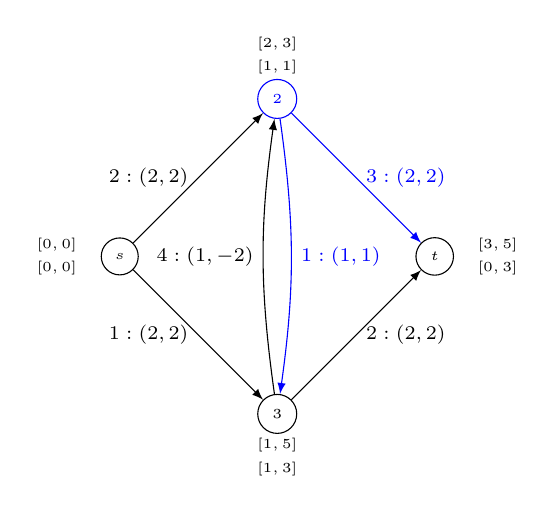
\begin{tikzpicture}[font=\tiny]
        %nodes
        \node at (-0.8, 0.15) {\blue{$[0,0]$}};
        \node at (-0.8, -0.15) {\blue{$[0,0]$}};
        \node[circle, draw] (s) at (0, 0) {\blue{$s$}};
        \node at (2, 2.7) {\blue{$[2, 3]$}};
        \node at (2, 2.4) {\blue{$[1, 1]$}};
        \node[blue, circle, draw] (a) at (2, 2) {\blue{$2$}};
        \node at (2, -2.4) {\blue{$[1, 5]$}};
        \node at (2, -2.7) {\blue{$[1, 3]$}};
        \node[circle, draw] (b) at (2, -2) {\blue{$3$}};
        \node at (4.8, 0.15) {\blue{$[3, 5]$}};
        \node at (4.8, -0.15) {\blue{$[0, 3]$}};
        \node[circle, draw] (t) at (4, 0) {\blue{$t$}};
        %edges
        \path [draw,-latex] (s) to node[left]{\scriptsize\blue{$2: (2, 2)$}} (a);
        \path [draw,-latex] (s) to node[left]{\scriptsize\blue{$1: (2, 2)$}} (b);
        \path [blue, draw,-latex] (a) to node[right]{\scriptsize\blue{$3: (2, 2)$}} (t);
        \path [draw,-latex] (b) to node[right]{\scriptsize\blue{$2: (2, 2)$}} (t);
        \path [blue, draw,-latex] (a) edge [bend left=8] node[right]{\scriptsize\blue{$1: (1, 1)$}} (b);
        \path [draw,-latex] (b) edge [bend left=8] node[left]{\scriptsize\blue{$4: (1, -2)$}} (a);
      \end{tikzpicture}
      \caption{Arcs explored the for loop at line \ref{step:explore_arcs} when \blue{$i = 2$}.}
      \label{fig:vrptw_disposable_example}
    \end{figure}
  \end{multicols}
\end{frame}


\begin{frame}
  \frametitle{Algorithm}
  \framesubtitle{Example}
  \begin{multicols}{2}
    State at the end of \blue{$4$}th iteration of the while at line \ref{step:main_while}:
    \begin{itemize}   
      \item \blue{$\Lambda_s = \{ ((0, 0, 1, 1, 0, 0, 0), 0) \}$};
      \item \blue{$\Lambda_2 = \{((3, 0, 3, 1, 1, 1, 0), 5)\}$};
      \item \blue{$\Lambda_3 = \{((2, 2, 2, 1, 0, 1, 0), 1)\}$};
      \item \blue{$\Lambda_t = \{((5, 2, 4, 1, 1, 1, 1), 8)\}$};
      \item \blue{$N = \emptyset$};
    \end{itemize}   
    \begin{figure}[H]
      \centering
      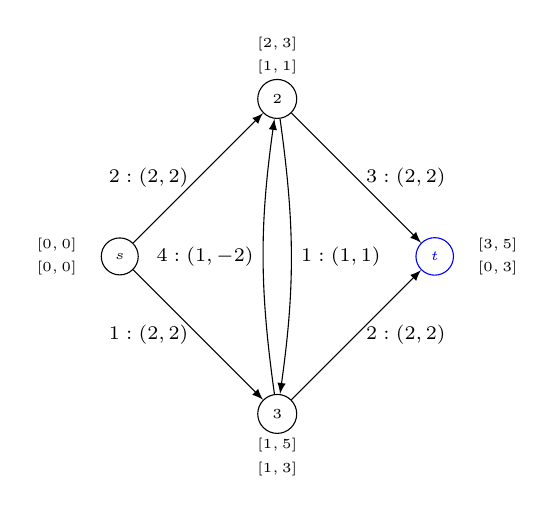
\begin{tikzpicture}[font=\tiny]
        %nodes
        \node at (-0.8, 0.15) {\blue{$[0,0]$}};
        \node at (-0.8, -0.15) {\blue{$[0,0]$}};
        \node[circle, draw] (s) at (0, 0) {\blue{$s$}};
        \node at (2, 2.7) {\blue{$[2, 3]$}};
        \node at (2, 2.4) {\blue{$[1, 1]$}};
        \node[circle, draw] (a) at (2, 2) {\blue{$2$}};
        \node at (2, -2.4) {\blue{$[1, 5]$}};
        \node at (2, -2.7) {\blue{$[1, 3]$}};
        \node[circle, draw] (b) at (2, -2) {\blue{$3$}};
        \node at (4.8, 0.15) {\blue{$[3, 5]$}};
        \node at (4.8, -0.15) {\blue{$[0, 3]$}};
        \node[blue, circle, draw] (t) at (4, 0) {\blue{$t$}};
        %edges
        \path [draw,-latex] (s) to node[left]{\scriptsize\blue{$2: (2, 2)$}} (a);
        \path [draw,-latex] (s) to node[left]{\scriptsize\blue{$1: (2, 2)$}} (b);
        \path [draw,-latex] (a) to node[right]{\scriptsize\blue{$3: (2, 2)$}} (t);
        \path [draw,-latex] (b) to node[right]{\scriptsize\blue{$2: (2, 2)$}} (t);
        \path [draw,-latex] (a) edge [bend left=8] node[right]{\scriptsize\blue{$1: (1, 1)$}} (b);
        \path [draw,-latex] (b) edge [bend left=8] node[left]{\scriptsize\blue{$4: (1, -2)$}} (a);
      \end{tikzpicture}
      \caption{Arcs explored the for loop at line \ref{step:explore_arcs} when \blue{$i = t$}.}
      \label{fig:vrptw_disposable_example}
    \end{figure}
  \end{multicols}
\end{frame}
